\section{Introduction}
\subsection{Background}
People have been playing mathematical games
since as early as 2000 B.C.
\cite{cornelius1986historical}.
All along,
players have attempted to devise optimal
strategies, simulate future moves, or identify
flaws that can be exploited.
Mathematics can serve as a particularly powerful tool for
such analysis.
Abbott and Richey used Markov Chains
to find the long term 
distribution of turns players spend in different
properties in the board game
\textit{Monopoly} \cite{abbott1997take, magie1935}.
(They also found that the optimal strategy is to avoid making
moves altogether and instead maximize time spent in jail.)
Lyford et al. investigated the probability and expected value 
in the board game \textit{Camel Up}
\cite{bogen2014, lyford2019using}.
Witter and Lyford generated an optimal winning strategy for the 
board game \textit{Codenames} using matrix rotations
and a combinatorial argument \cite{chvatil2015}.
% TO DO: CITE CODENAMES PAPER IF ACCEPTED

Another example of a game with mathematical underpinnings is
the board game \textit{Ticket to Ride} \cite{moon2004ticket}. 
Players race to connect 
cities and build railroads on a map of the U.S.
Mathematically, the board
can be thought of as a graph where
cities represent vertices and the
routes between them represent edges.
The educational implications of \textit{Ticket to Ride}
have been extensively studied.
Lim applied the game to teach basic graph theory
\cite{lim2007taking}.
Chang et al. introduced Kruskal's, Prim's, and Dijkstra's
algorithms in the context of \textit{Ticket to Ride}
\cite{chang2008learning}.
Finally, Drake taught beginning programming skills by having
students implement a digital version of the game \cite{drake2011teaching}.
In addition, \textit{Ticket to Ride} has been studied in the context of
accessible game design and eye-tracking visualization
\cite{eriksson2005enhancing, newn2017evaluating}.

Previous work has also focused on improving player 
strategies in \textit{Ticket to Ride}.
Silva et al. used simulations to compare different
heuristic strategies (e.g. purchasing longest routes,
connecting all destination cards, etc.) \cite{de2017playtesting}.
In related papers, the same authors explore the 
game space to find trends in the way \textit{Ticket to Ride}
is played and experiment with new maps and decks 
\cite{de2017evaluator, de2018evolving}.

We extend the mathematical interpretations of
\textit{Ticket to Ride} to build on previous research
and devise better player strategies.
In particular, we apply expected value of collecting cards,
effective resistance, and betweenness centrality to
analyze the game.

To investigate a better way to assign points for building routes,
we rely on a well-known solution to the probability question:
"What is the expected number of cards until
we see three aces in a well-shuffled deck?"
We frame the problem of collecting the resources
to build a route in terms of the aces problem
and use the solution to gives a proxy for the difficulty
of collecting routes.

To investigate the difficulty of connecting pairs of cities,
we use effective resistance.
In graph theory, effective resistance is a measure of the 
difficulty an electrical flowing from one node to another faces.
We implement two existing algorithms to calculate
the effective resistances between cities
\cite{ellens2011effective, wu2004theory}
and apply them to the Laplacian of the graph in \textit{Ticket to Ride}.
By comparing the effective resistance to the reward
of collecting a pair of cities, we suggest
strategies for players to pick destination cards.

To investigate the most important routes to own,
we use betweenness centrality.
Developed in 1977, betweenness centrality gives a measure
of how central edges are to a graph
\cite{freeman1977set}.
By calculating the edges with the highest betweenness centrality,
we enable players to pick the most central routes.
In addition, we compare the most theoretically central routes
to the ones owned by the winning player in Silva et al.'s
simulations \cite{de2017playtesting}.

The overarching question of this work is as follows:
What (if any) mathematical structure in \textit{Ticket to Ride}
can be exploited to optimize player strategies?
Our answer builds on existing results and
and our own novel applications of mathematical concepts to enhance
player strategies and propose a better scoring scheme.

\subsection{\textit{Ticket to Ride} Gameplay}

The goal of \textit{Ticket to Ride} is to collect
the most points by the end of the game.
There are three ways players may accumulate points:
First, a player receives points for building routes
on the board in \cref{fig:board}.
The number of points scored is based on the length of the route
according to  \cref{table:current_value}.
Second, a player receives points for building
a set of routes that connect two cities in proportion
to the number of trains along the shortest path between cities.
(Points may only be scored for a pair of cities specified by a 
Destination Ticket in the player's hand.)
Finally, a player receives points for building
the longest path of cities at the end of the game.
(A path connects two cities through a set
of routes and may only use a single route exactly once.)

\begin{figure}[H]
\centering
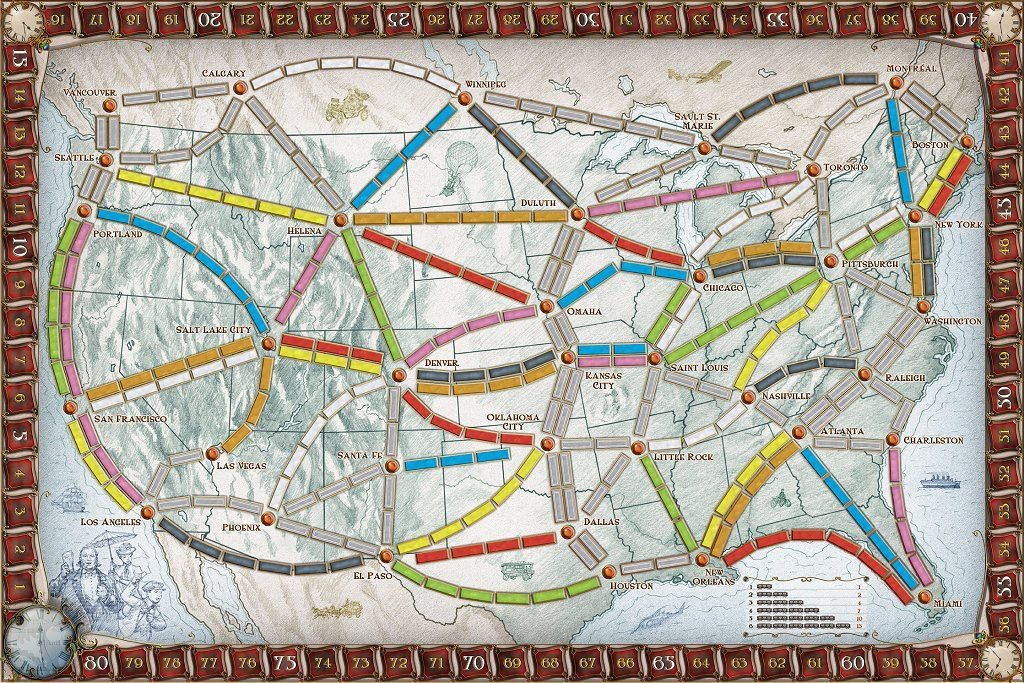
\includegraphics[scale=.2]{figures/board}
\captionof{figure}{The \textit{Ticket to Ride} U.S. board.}
\label{fig:board}
\end{figure}

Each player begins the game with four random Train Car cards.
These cards are used to buy routes.
For example, a player can use four pink Train Car cards to purchase
the route between Charleston and Miami
(at the bottom right corner of \cref{fig:board}).
At the beginning of the game 
each player also receives three Destination Ticket cards.
Two cities and a reward are specified on each Destination Ticket.
Players choose either two or three of these cards and
receive points at the end of the game based on whether
or not they completed the Destination Ticket:
if they connected the cities then they add the point reward to their
total score and
if they did not connect the cities they subtract the points from their
total score.

Players take one of three actions on their turns.
First, a player may draw two Train Car cards either
from the deck or from the five Train Car cards
kept face up on the table. 
(If a player chooses a wild card from the table
then they are limited to one Train Car card that turn.)
Second, a player may claim a route by trading in
the appropriate number and color of Train Car cards.
The gray routes on the map are purchased with
the appropriate number of any one color.
If a pair of cities have two routes between them,
no player can claim both.
Finally, a player may draw three Destination Tickets
and return up to two of them.

When one player's stock of 45 trains dips below 3 trains at the end of their turn,
every player (including that player) gets one final turn.

\subsection{Simulations}
We used Silva et al.'s program to simulate
\textit{Ticket to Ride} games \cite{silva2019}.
We run our simulations on the regular U.S.A. map.
For four-player games, we include each of Silva et al.'s 
four agent types:
The Destination Hungry Agent chooses 
Destination Tickets at the beginning of the
game--with an emphasis on Destination 
Tickets that are geographically close--
and tries to connect them for the rest of the game.
The Route Focused Agent works toward a longer Destination Ticket then
claims longer routes.
The One Step Agent operates by choosing the most advantageous move at each
step without a long term strategy.
The Long Route Agent claims longer routes (defined as four trains or more)
with a preference for routes that help 
connect the player's initial Destination Tickets.
For two-player games, we simulate an equal number 
of all six pairings of the four agents.
Our forked verision of Silva et al.'s
Github repository is publicly available online
\cite{witter2019}.

\subsection{Overview}
\todo{view over}
